%\documentclass[a4paper,oneside,11pt]{book}
\documentclass[a4paper,11pt]{book}
\usepackage[dutch]{babel}
\usepackage{textcomp}
\usepackage{fancyhdr}
\usepackage{makeidx}
\usepackage{tabularx}
\usepackage{LTXtable}
\usepackage{graphicx}
\usepackage{parskip}
\usepackage{pdflscape}
\usepackage{floatflt}
\makeindex
\pagestyle{fancy}
\fancyhf{}
%\fancyhead[L,RO]{\bfseries\thepage}
%\fancyhead[LO]{\bfseries\rightmark}
%\fancyhead[R]{\bfseries\leftmark}
\rhead[]{\bfseries \leftmark}
\lhead[\bfseries \leftmark]{}
\rfoot[]{\thepage}
\lfoot[\thepage]{}
\renewcommand{\headrulewidth}{0.5pt}
\renewcommand{\footrulewidth}{0pt}
\addtolength{\headheight}{0.5pt}
\fancypagestyle{plain}{%
	\fancyhead{}
  \lhead[thesection]{\bfseries}
  \rfoot[thesection]{\thepage}
	\renewcommand{\headrulewidth}{0pt}
}
\usepackage[pdftex,pdfstartview=FitV]{hyperref}
\hypersetup{%
  pdftitle={Stageverslag: HSB Bus Analyzer},%
  pdfauthor={Rink Springer},%
  pdfkeywords={Stage Fontys XML CAN HSB Delem}
}
\hyphenation{super-klasse hoofd-feature pro-ject-be-schrij-ving il-lu-stra-tie tekst-be-stan-den}

% definities
\author{Rink Springer}
\title{Stageverslag}

\begin{document}

\frontmatter

% titel pagina
\begin{titlepage}
\hrule
\vspace*{\fill}
\begin{center}
{\Huge Stageverslag} \\
\vspace{2cm}
\begin{figure}[htb]
\begin{center}
\includegraphics[height=2cm]{delem_logo.jpg}
\end{center}
\end{figure}
HSB-Bus-Analyser\\
\vspace{2cm}
{\large Rink Springer}\\
\vspace{2cm}
Versie 1.2.1\\
\today\\
\vspace{2cm}
\end{center}
\vspace*{\fill}
\hrule
\vspace*{\fill}
\end{titlepage}

% voorblad
\thispagestyle{empty}
\begin{flushleft}
\textbf{STAGEVERSLAG VOOR FONTYS HOGESCHOOL INFORMATICA}
\textbf{TWEEDE STAGE}
\begin{tabular}{ll}
&
\tabularnewline
\tabularnewline
\textbf{Gegevens Student:}&
\tabularnewline
\tabularnewline
\hline 
&
\tabularnewline
Naam:&
Springer, R.P.W. ( Rink )\tabularnewline
Studentnummer:&
2016014\tabularnewline
Opleiding:&
Hogere Informatica\tabularnewline
&
Voltijd\tabularnewline
&
\tabularnewline
Stageperiode:&
02/02/2004 - 18/06/2004\tabularnewline
&
\tabularnewline
\textbf{Gegevens Bedrijf:}&
\tabularnewline
\tabularnewline
\hline 
&
\tabularnewline
Naam bedrijf:&
Delem B.V.\tabularnewline
Afdeling:&
Development\tabularnewline
Plaats:&
Eindhoven, Nederland\tabularnewline
Naam bedrijfsbegeleider:&
M. Scholte\tabularnewline
&
\tabularnewline
\textbf{Gegevens Docentbegeleider:}&
\tabularnewline
\tabularnewline
\hline 
&
\tabularnewline
Naam docentbegeleider:&
J.B.H.M. van Heumen\tabularnewline
&
\tabularnewline
\textbf{Gegevens verslag:}&
\tabularnewline
\tabularnewline
\hline 
&
\tabularnewline
Titel Stageverslag:&
HSB Bus Analyzer\tabularnewline
Datum uitgifte stageverslag:&
07/06/2004\tabularnewline
&
\tabularnewline
\hline 
\tabularnewline
Getekend voor gezien door bedrijfsbegeleider:&
\tabularnewline
\tabularnewline
&
\tabularnewline
Datum:&
\tabularnewline
\begin{tabular}{|p{2in}|}
\hline 
\tabularnewline
\tabularnewline
\hline
\end{tabular}&
\tabularnewline
&
\tabularnewline
De bedrijfsbegeleider,&
\tabularnewline
&
\tabularnewline
\end{tabular}\end{flushleft}


% voorwoord
\section{Voorwoord}
\index{Voorwoord}

Dit Plan van Aanpak is geschreven tijdens mijn 2$^{e}$ stage bij de firma Delem. Het doel is de betrokkenen te informeren over mijn aanpak van het project en is in de eerste instantie bestemd voor mensen die in direct verband met de stage staan. Uiteraard is het ook voor ge\"interesseerden toegankelijk.

\index{Conclusie}
Ik wil iedereen die mij tijdens mijn stage geholpen heeft, heel erg bedanken. Hierbij in het bijzonder de heer M. Scholte, die mij als bedrijfsbegeleider op weg helpt binnen het bedrijf en de heer H. van Heumen, die als stagebegeleider namens Fontys Hogescholen te Eindhoven optreedt.


\tableofcontents

% samenvatting
\chapter{Samenvatting}
\index{samenvatting}

Dit verslag biedt een overzicht van mijn afstudeerstage bij Philips Research. Het directe resultaat is een Linux filesysteem dat direct in de Linux kernel opgenomen kan worden, programma's om het filesysteem aan te maken, te controleren en te debuggen. Tot slot is er een rapport geschreven dat de technische aspecten van het filesysteem belicht en een het uiteindelijke afstudeerverslag dat u nu aan het lezen bent.

Tijdens de stage heb ik erg diep in de Linux kernel gekeken, waarbij vooral de filesystemen en het I/O systeem centraal stond. Het resultaat hiervan is kennis over de interne Linux kernel structuren, die zeker van pas zullen komen in de toekomst. Verder heb ik ook de Extreme Programming-methode erg veel toegepast.


% summary
\chapter{Summary}
\index{summary}

This report provides an in-depth view of the technical aspects of the LIMEFS filesystem. It provides an extensive overview of the LIMEFS filesystem as well as a brief overview of the Linux Virtual File System design.

The following aspects are covered by this report:

\begin{itemize}
\item Linux I/O Layer \\
What is the basic design, what does a filesystem have to provide? Focuses mostly on the Linux Virtual File System layer.
\item LIMEFS \\
Overall design ideas of the LIMEFS filesystem, as well as all structures used within the LIMEFS filesystem.
\item Implementation \\
Linux Implementation-specific details of the filesystem.
\end{itemize}

The overall conclusion of the report is a stable filesystem which is very suitable for storing large files of a few gigabytes. There is room for improvement, especially within the administration part of the filesystem. As for most multimedia applications, the filesystem is ready to be used.


% verklarende woordenlijst
\thispagestyle{empty}
\chapter{Verklarende woordenlijst}
\index{Verklarende woordenlijst}
\label{woordenlijst}

\LTXtable{\textwidth}{woorden.tex}


\mainmatter

% 1. inleiding
\chapter{Inleiding}
\index{Inleiding}

Vlakbij Eindhoven Airport, aan de Luchthavenweg zit de firma Delem. Dit is een bedrijf dat zich richt op het ontwerpen en produceren van besturingen van drukpersen ten behoeve van metaalbewerking. Van februari tot juni 2004 heb ik stage gelopen bij de afdeling Development.

Er werken ongeveer 60 mensen bij Delem, waarvan ongeveer 30 in de afdeling Development. De overige werknemers werken bij de productie, sales en ondersteunende
afdelingen.

Gezien Delem zich in een zeer gespecialiseerde markt bevind, is kwaliteit afleveren zeer belangrijk. Maar minstens zo belangrijk is het bewaken van deze kwaliteit. Dat is in principe de essentie van deze opdracht, die in hoofdstuk 2 op pagina \pageref{opdracht} verder beschreven zal worden.

Daarna zullen vervolgens de onderzoeken, het proces, de implementatie en uiteindelijk de conclusie volgen. Elk hoofdstuk geeft een kijk op een ander deel van de stage, waarbij de conclusie vanzelfsprekend een afsluitende kijk op het geheel geeft.


% 2. het proces
\chapter{Proces}
\index{Proces}
\label{proces}

Dit hoofdstuk beschrijft het ontwikkelproces van deze stage. Hierbij zal de manier van werken centraal staan, alswel het verloop.

\section{Projectmanagement}
\index{projectmanagement}

Zoals in het Plan van Aanpak vermeld staat (in het de paragraaf fasering op bladzijde \pageref{fasering}), is binnen Delem elk project opgedeeld in zogenaamde \index{Milestones}\emph{milestones}. Voor dit project is elke milestone weer opgedeeld in zogenaamde \index{Increments}\emph{increments}, een periode van twee weken. Hierbij stond elke increment een hoofdfeature centraal. Dit zal in de overzichten op de pagina's hierna te zien zijn.

Dit is te vergelijken met het standaard \index{waterval model}waterval model:

\begin{figure}[h]
\includegraphics[width=\textwidth]{waterval}
\end{figure}

Het grootste verschil met het standaard waterval model, is dat nu het model meerdere keren doorlopen wordt (namelijk \'e\'en waterval per increment). Verder wordt aan het begin van elke increment naar de requirements gekeken, in tegenstelling tot eenmalig aan het begin van het project. Tenslotte is de terugkoppeling met de gebruikers iets waarin het 'standaard' watervalmodel helemaal niet voorziet.

\section{Besprekingen}
\index{Besprekingen}

Na een gesprek met de bedrijfsbegeleider, besloten we elke maandag een uur te vergaderen over het project. Hierbij stonden de volgende zaken centraal:

\begin{itemize}
\item Voortgang \\
Wat is er van de zaken die vorige keer besproken zijn terecht gekomen?
\item Toekomst \\
Wat is de bedoeling voor volgende weken?
\end{itemize}

Deze aanpak is gekozen, omdat de uiteindelijke \index{requirements}requirements van het project (dus een concrete lijst wat het moet kunnen) niet beschikbaar was. Vanuit Delem was het idee om ontwikkelaars het programma te laten gebruiken en aan de hand van het commentaar erop het te laten groeien. Zo kwam er een programma precies volgens de wensen van de ontwikkelaars (dit is prima omdat het voor intern gebruik is)

Na elke increment is er gekeken naar wat we nu hadden en wat de bedoeling was om eraan toe te voegen. Zo kwam er op de uiteindelijke planning naar voren dat er halverwege increment 6 weinig meer aan toe te voegen was, omdat er geen nieuwe requirements waren die ge\"\i mplementeerd moesten worden.

Om het verloop zo goed mogelijk weer te geven, is er op de volgende bladzijde de initi\"ele planning te zien en op de bladzijde daarna het definitieve resultaat van de planning.

\begin{landscape}

\section{Initi\"ele Planning}
\index{Planning!Initi\"ele}

Dit is de initi\"ele planning. Kenmerkend is, dat er weinig vooruit gepland is, omdat we niet teveel op de zaken vooruit wilden lopen. Dit omdat er in dit stadium weinig bekend was over de gewenste functionaliteit.

\begin{figure}[h]
%\includegraphics[width=20cm,height=9.5cm]{initiele_planning.png}
\includegraphics[width=15cm]{initiele_planning.png}
\end{figure}

\newpage

\section{Definitieve Resultaat}
\index{Resultaat!Definitieve}

Uiteindelijk is dit de realiteit geworden. Kenmerkend is, dat bijvoorbeeld de hele Cycle Viewer increment eruit gevallen is, omdat achteraf bleek dat de persbesturing deze functionaliteit al bevatte.

\begin{figure}[h]
\includegraphics[width=20.9cm,height=9.7cm]{def_res.png}
\end{figure}

\end{landscape}


% 3. de opdracht
\chapter{De opdracht}
\index{opdracht}
\label{opdracht}

De opdracht van deze stage was het ontwerpen en implementeren van een applicatie die verkeer op de \index{CAN}CAN Bus van Delem besturingen kan analyseren en kwalificeren. De exacte invulling van deze opdracht werd tijdens de stage zelf ingevuld, aan de hand van feedback van de ontwikkelaars.

Dit had tot gevolg dat de tool zo breed en uitgebreid mogelijk opgezet diende te worden, zodat er altijd meer bijgebouwd kon worden. Een eis was wel, dat bestaande uitvoer van de Warwick X-Analyzer tool gelezen moest kunnen worden, alsmede real-time analyse door middel van een Softing CANusb en CANcard device.

Een groot probleem was het verzuimen tot updaten van documentatie. Steeds als er nieuwe commando's op de bus bijgevoegd werden, werd vaak de documentatie niet netjes up-to-date gebracht. Na verloop van jaren was er dus vrij veel niet meer duidelijk.

Om dit verschijnsel tegen te gaan, moest er een makkelijk uitbreidbare definitie van commando's bedacht worden. De bedoeling was om deze definitie zo makkelijk mogelijk door ontwikkelaars zelf te laten aanpassen, terwijl vanuit deze definitie de benodigde structuren gegenereerd werden die het programma begreep. Een voorstel voor het formaat hiervan was \index{XML}XML\footnote{Extensible Markup Language, een markup taal met zelf defini\"eerbare elementen}.

Daarnaast werd het idee geopperd, om aangezien er toch een duidelijke definitie bestaat, ook direct documentatie te genereren vanuit deze definitie. Er bestond een Microsoft Word document, maar na verloop van tijd was dit hopeloos verouderd. Het idee achter het genereren van documentatie vanuit de definitie is: als het niet in het gegenereerde document staat, herkent de applicatie het commando ook niet en bestaat het commando logischerwijs niet.

Het kwalificerende deel van de applicatie moet in staat zijn om mee te lopen tijdens het testen van de besturingssoftware. Mochten er dan problemen optreden tijdens het testen, moet er aan de hand van de log van de applicatie uitgezocht kunnen worden of er vreemde of ongeldige berichten op de HSB bus geweest waren. Deze logs moeten dus leesbaar in de applicatie zijn, zodat eventuele problemen snel geanalyseerd kunnen worden.

De initi\"ele bedoeling was om ook een cyclus viewer te maken, die elke fase van het persen in beeld kon brengen. Nadat dit aan de ontwikkelaars voorgelegd was, bleek dat de besturing deze functionaliteit al had en het absoluut niet nuttig zou zijn om dit te implementeren.

Tenslotte was het ook de bedoeling, om ontwikkelaars zo makkelijk mogelijk zaken te laten toevoegen aan de applicatie. Mocht er een zeer specifiek probleem zijn om te debuggen, dan was het zeker niet de bedoeling om de hele applicatie opnieuw te moeten bouwen. Om hierin te voldoen is er een plugin structuur bedacht, waar door middel van DLL files extra functionaliteit toegevoegd kan worden.


% 4. de onderzoeken
\chapter{Onderzoek}

Zoals in de opdrachtomschrijving op pagina \pageref{opdracht} te zien is, was het noodzakelijk om een aantal onderzoeken uit te voeren, aan de hand van welke besluiten genomen konden worden. In dit hoofdstuk komen al deze onderzoeken aan bod, met hun uitvoering en conclusies.

\section{CAN Hardware}

Een van de eerste onderzoeken was een analyse van de huidig beschikbare CAN hardware, die de verbinding tussen de CAN bus en de PC verzorgen.

Een eis was wel, mocht er ooit besloten worden andere hardware aan te schaffen, het mogelijk moest zijn hier makkelijk een driver voor te maken. Dit is opgelost door een generieke architectuur te ontwerpen, die later toegelicht zal worden.

Op internet heb ik de specificaties opgezocht van een aantal leveranciers van CAN hardware en hiervan een duidelijk overzicht gemaakt. Ook de \index{API}API werdt hierbij onder de loep genomen, om er zeker van te zijn dat software daadwerkelijk aansloot bij de hardware.

De uiteindelijke conclusie hier was, dat de huidige Softing CANusb dongel prima geschikt was voor de Delem toepassingen. Er waren veel luxere en minder luxe te krijgen, maar omdat er hier al enkelen van in het bezit van Delem zijn, is er besloten deze te gebruiken.

\section{Definitie}
\label{definitie}

Zoals in de opdrachtomschrijving te vinden is, was een verdere eis het omschrijven van de HSB commando's in een eenvoudig formaat. Dit formaat moest makkelijk uitbreidbaar zijn, zonder in de knoop te raken met bestaande definities.

Om dit te realiseren werd door een ontwikkelaar \index{XML}XML voorgesteld. Om te kijken of die geschikt was, is er eerst gekeken wat voor zaken er gespecifeerd dienden te worden om alle commando's eenduidig te kunnen identificeren.

Nadat dit bekend werd, is er een voorbeeld XML bestand gemaakt met wat commando's erin en via \index{XSLT}XSLT omgezet naar C structuren, die door een preprocessor module toegepast word op de inkomende gegevensstroom.

De versie die dit ondersteunde is omgedoopt tot prototype en is uitvoerig besproken met de bedrijfsbegeleider. Deze was dusdanig enthousiast dat er besloten is op deze manier door te gaan.

Hierna is er gekeken om deze definities ook naar HTML te converteren, als documentatie. Toen later bleek dat je met een HTML bestand en een HHC\footnote{Inhoudsopgave bestand voor een CHM file} file een CHM file kan maken is ervoor gekozen om dit als help formaat binnen de applicatie te gebruiken, zodat commando's makkelijker op te zoeken zijn.

Het was uiteindelijk ook de bedoeling om het bestaande document met commando's te kunnen genereren vanuit de definitie. Dit overzicht zal aan het bestaande document toegevoegd worden, als een appendix. De definities worden weer door XSLT geprocessed, maar dan naar \LaTeX\mbox{-}formaat. Dat laatste wordt door \LaTeX\mbox{-}uiteindelijk geprocessed naar een PDF bestand, dat netjes uit te printen is.

Later is er ook gekeken naar de mogelijkheid om deze definities rechtstreeks uit de XML file zelf te lezen. Na een korte vergelijking tussen MSXML en libxml2 is er gekozen voor de laatste, aangezien MSXML zeer omslachtig in het gebruik is. Verder is de documentatie van libxml2 veel beter en kon er meteen mee aan de slag worden gegaan. Het resultaat is dat je definities voortaan kunt aanpassen zonder het programma opnieuw te moeten compileren.

\newpage
\subsection{Overzicht}

Uiteindelijk ziet het overzicht van het XML-transformatie proces er als volgt uit:

\begin{figure}[h]
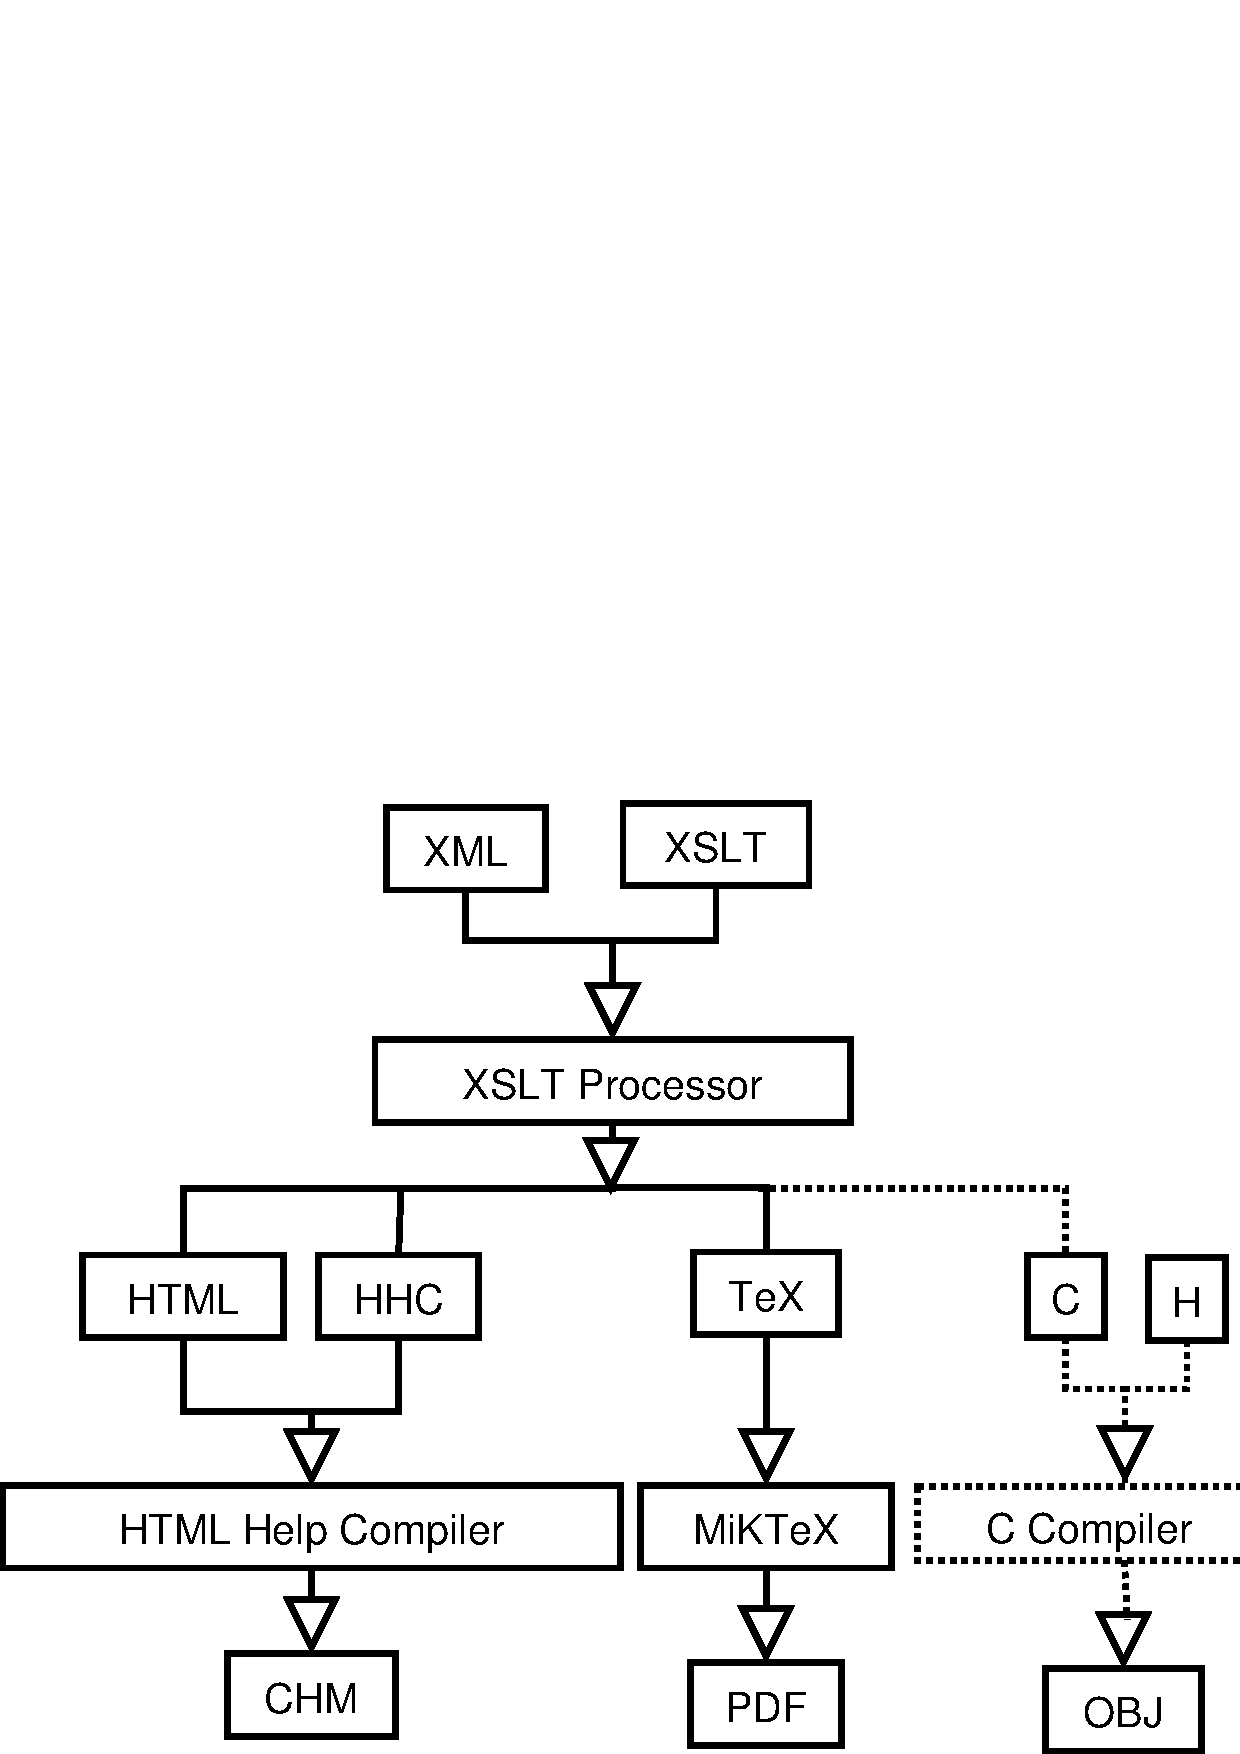
\includegraphics[width=\textwidth]{xml.pdf}
\end{figure}

In dit overzicht is het C-gedeelte met stippellijnen aangeduid, omdat dit stuk later kwam te vervallen.

\section{Uitbreidbaarheid}

Aan het einde van het project bleek dat er een extreem grote behoefte was tot het eenvoudig ontwikkelen van plugins, die ervoor zorgen dat de huidige functionaliteit eenvoudig uit te breiden is. Er werden twee mogelijkheden bekeken: scripts en DLL bestanden.

Het voordeel van scripts was dat ze erg makkelijk te maken en onderhouden zijn. Helaas was de verwachting dat het realtime gedrag niet meer gegarandeerd kan worden als er voor een dusdanige oplossing gekozen zou worden. Daarom is deze oplossing verder dus niet verder onderzocht.

DLL bestanden leken ideaal: het is gewoon C++ code, je kunt bestaande code recycelen. Nadat er dan ook een goede API ontworpen was, die later flink uitgebreid is, is dit dan ook gepresenteerd aan de ontwikkelaars. Deze API werkt prima en er zijn geen verschillen bemerkbaar in snelheid.


% 5. de implementatie 
\chapter{Implementatie}
\index{Implementatie}

Dit hoofdstuk presenteert een overzicht van de implementatie van de applicatie. Hierbij komt de interne opzet van het programma naar voren. De gebruikte software is opgenomen als een bijlage die te bekijken is op pagina \pageref{software}.

\begin{landscape}

\section{Ontwerp}
\index{Ontwerp}
\label{ontwerp}

Aangezien de applicatie in principe een datastroom moet analyseren en eventueel weergeven, moet het ontwerp beschrijven hoe data door de applicatie heen stroomt. Zie het volgende plaatje:

\begin{figure}[h]
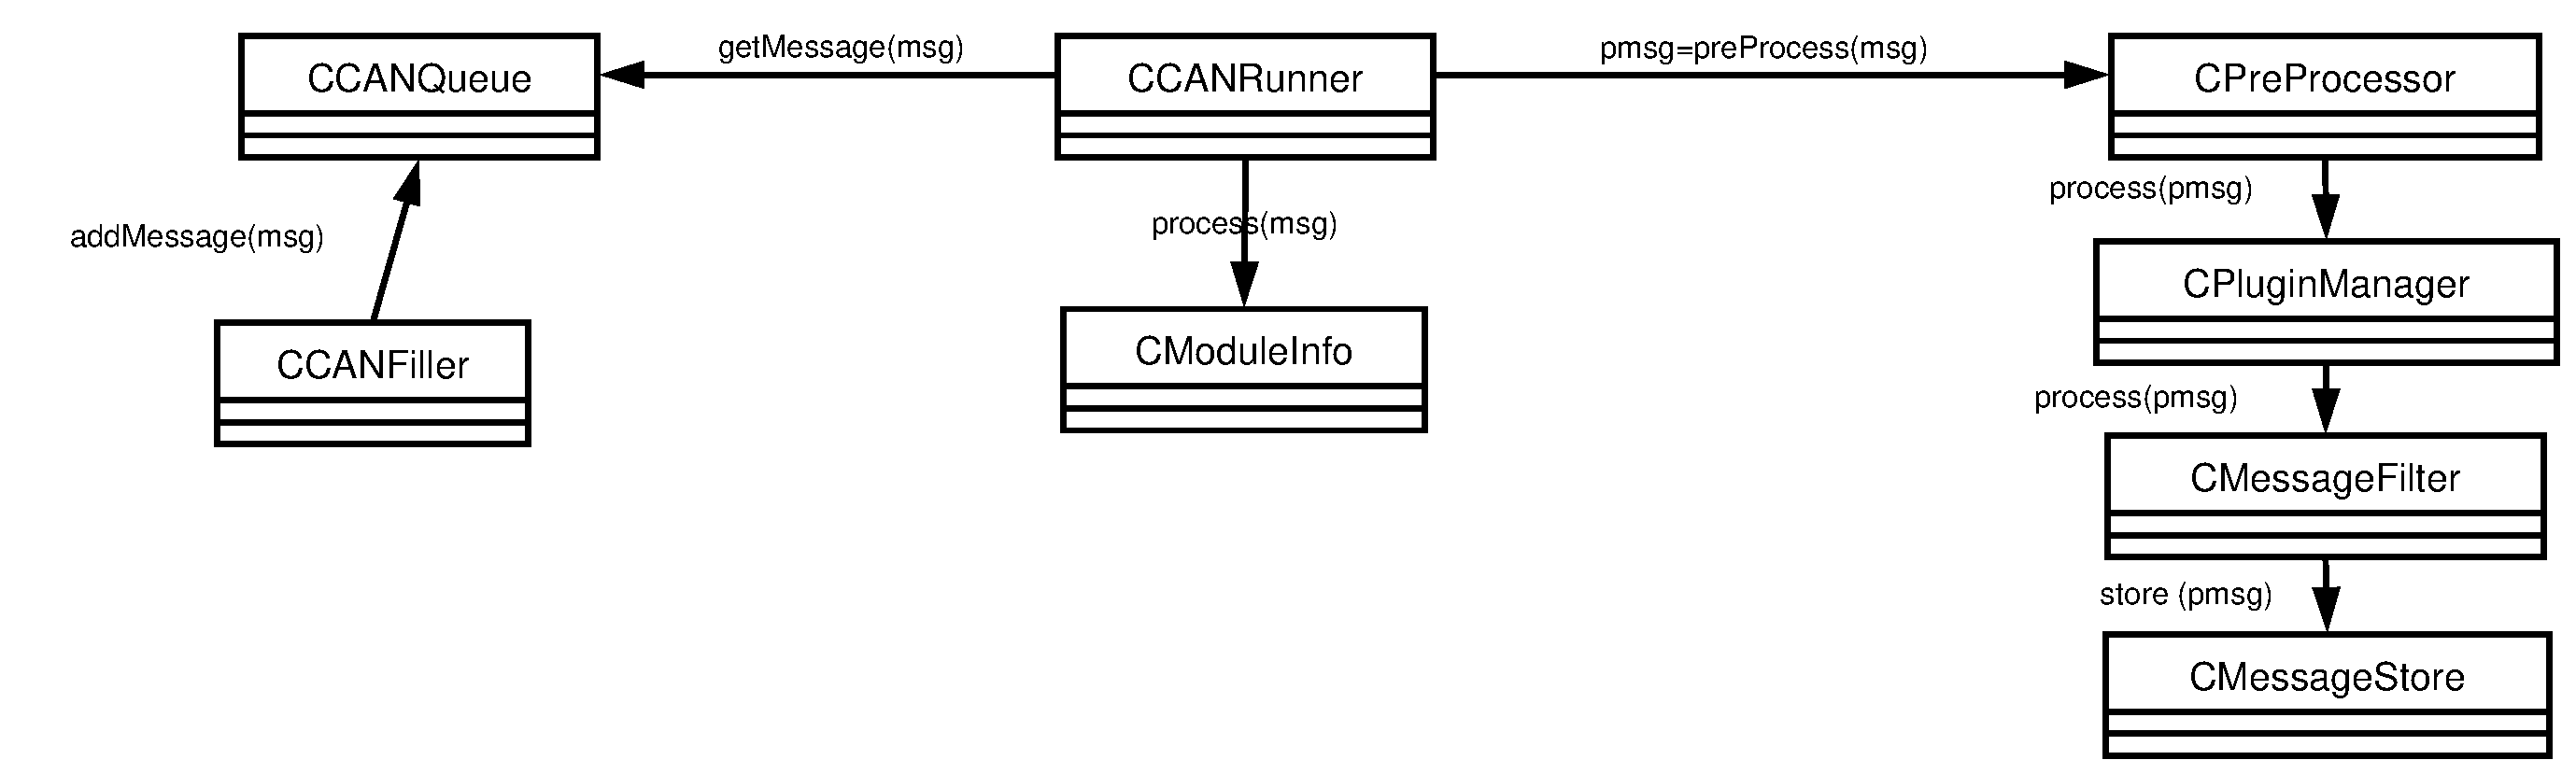
\includegraphics[width=18cm,height=6.5cm]{dataflow}
\end{figure}

Omdat het hier alleen de datastroom beschrijft en verder geen directe interfacing, is er gekozen voor een eenvoudigere representatie dan UML. De insteek is om de dit diagram ook leesbaar te laten zijn voor mensen die geen kennis van de zogenaamde use-cases hebben.

\end{landscape}

De berichten worden in principe opgebouwd door een \emph{CCANFiller} superklasse. Deze klasse zorgt ervoor, dat berichten van een bron (zoals de CAN hardware, maar bijvoorbeeld ook berichten uit een bestand) opgeslagen worden in een zogenaamde \emph{CCANQueue}. Om ervoor te zorgen dat het ontvangen, bewerken en weergeven synchroon van elkaar gebeurd, bevindt de \emph{CCANFiller} zich in een eigen thread.

Alle te behandelen berichten komen dus in de \emph{CCANQueue}. Deze klasse wordt door middel van \index{Mutex}mutexes beschermd tegen \index{deadlock}deadlocks en dergelijke, gezien hij door meerdere threads tegelijk word gebruikt.

De \emph{CCANRunner} superklasse wacht net zo lang tot de \emph{CCANQueue} een bericht teruggeeft dat behandeld dient te worden. Zoals reeds vermeld gebeurt het afhandelen in een aparte thread. Het enige dat de \emph{CCANRunner} doet is de berichten door alle subsystemen heen voeren.

Tijdens het verwerken worden de berichten eerst door de \emph{CModuleInfo} klasse gevoerd. Deze kijkt of er modules op de HSB bus toegevoegd of aangepast moeten worden. Dit gebeurd voor de daadwerkelijke verwerking op bericht-niveau, aangezien bepaalde typen berichten (de zogenaamde sequencer berichten) pas geidentificeerd kunnen worden als het moduletype bekend is. Aangezien deze klasse nooit het bericht uitbreidt, maar alleen de interne module administratie, is dit als een aparte pijl getekend in het diagram op de vorige pagina.

Nu komt de klasse die daadwerkelijk de berichten behandelt: de \emph{CPreProcessor} klasse. Deze klasse breidt de bestaande, rauwe bericht-data uit aan de hand van de definities in de ingelezen XML file. De uitvoer van deze klasse bevat dan ook het complete rauwe bericht met daarin ook de commandoinformatie, de argumenten, de bijbehorende module enzovoorts.

Deze informatie wordt aan de \emph{CPluginManager} klasse doorgegeven, die eventuele plugins de mogelijkheid geeft om de data verder te analyseren en gegevens ten behoeve van logging eraan toe te voegen. De berichtenstroom kan normaliter niet veranderd worden (tenminste, niet zonder er speciale moeite voor te doen). De plugins van de \emph{CPluginManager} klasse kunnen aangeven dat iets geforceerd gelogd moet worden en met welke melding dat moet.

Aangezien nu alle behandeling gereed is, rest het de \emph{CMessageFilter} klasse om te kijken of berichten gelogd moeten worden. Als de \emph{CPluginManager} of \emph{CPreProcessor} iets specifieks te melden hebben, dan wordt het bericht altijd gelogd.

Wanneer een bericht geschikt is bevonden om te loggen, dan wordt het uiteindelijk aan de \emph{CMessageStore} toegevoegd. Dit is een buffer die berichten kan bewaren. Het gebruikersinterface staat rechtstreeks in verbinding met deze klasse, zodat berichten niet dubbel opgeslagen hoeven te worden.

\section{Documentatie}

Sinds het begin van het project heb ik aangegeven eigen idee\"en te hebben over hoe het project gedocumenteerd kon worden. Dit is dan ook met mijn bedrijfsbegeleider besproken, waarna we uiteindelijk tot de volgende opzet kwamen:

\begin{itemize}
\item Code documentatie via Doxygen \\
Met behulp van het reeds genoemde Doxygen programma is er aan de hand van speciale constructies in de code documentatie gemaakt. Hiermee was snel op te zoeken wat een klasse of functie doet, welke in- en uitvoer die heeft, enzovoorts.
\item Architectuur Model in Microsoft Word \\
In het architectuur model staat het ontwerp van het programma uitgelegd. Dit lijkt erg veel op het ontwerp op bladzijde \pageref{ontwerp}, maar is veel meer toegespits op de code. De nadruk ligt dan ook op de link tussen functionaliteit van het programma en de code die het verzorgt.
\end{itemize}

Het architectuur model is later gereviewd door ontwikkelaars, waarna er uiteindelijk een duidelijk document uitkwam.


% 6. conclusie / aanbevelingen
\chapter{Conclusie}
\index{Conclusie}

Dit verslag bied een overzicht van het verloop van mijn werkzaamheden tijdens mijn $2^e$ stage te Delem BV. Na het gehele verloop van de stage is er een programma gemaakt, waarvan ik hoop dat Delem er veel aan zal hebben. De opzet was het programma zo uitbreidbaar en onderhoudbaar mogelijk te maken, iets wat goed gelukt is.

Tijdens deze stage heb ik, behalve aan de stageopdracht te werken, ook ongeveer \'e\'en dag per week aan andere activiteiten besteed. Een goed voorbeeld hiervan is het testen van een bestaande applicatie VBend\footnote{Virtual Bend, applicatie die een optimale buigvolgorde kan berekenen en simuleren}, waarvan binnenkort een nieuwe versie beschikbaar zou komen. Hierbij ben ik volledig in het projectteam opgenomen en heb ik goed kennis leren maken met de gang van zaken tijdens 'normale' projecten. Ook kwam het gebruik van \index{PR}PR's en \index{CR}CR\footnote{Problem Report/Change Request, zie pagina \pageref{PR} voor meer informatie}'s erg goed naar voren.

Verder heb ik tijdens deze stage heel uitgebreid kennis gemaakt met XML, wat wellicht later nog van pas kan komen. Ook merkte ik dat mijn Windows programmeerkennis niet meer optimaal was (ik gebruik zelf thuis bijna geen Windows), daarin heb ik mezelf ook een stuk meer verdiept.

Ik vind dat ik veel vrijheid heb gehad tijdens het uitoefenen van de stage, ik verwacht dat dit is omdat ik inmiddels al 2 jaar bij de firma Delem werkzaam ben. Hierbij ben ik van mening dat ik nu pas het bedrijf echt goed heb leren kennen, gezien ik eigenlijk pas nu het gevoel heb dat ik weet hoe de projecten daar werken .

Tenslotte denk ik dat dit een geslaagde stage was. Het is goed gedocumenteerd, er is een goed functionerend programma opgeleverd en er zijn al een aantal problemen mee gevonden die wellicht in de toekomst aangepakt zullen worden. Al met al een prima resultaat, wat ook door mijn projectbegeleider bij Delem bevestigd is.


% 7. bronvermelding
\chapter{Bronvermelding}
\index{Bronvermelding}

Hoogland, W., \emph{Rapport over Rapporteren}. $3^e$ druk, Groningen, 1998 \\
\\
Nederlands Computerwoordenboek, http://computerwoorden.nl


\appendix

% a. plan van aanpak
\chapter{Plan van Aanpak}

Deze bijlage bevat het plan van aanpak. Hierbij is de woordenlijst komen te vervallen, sinds het stageverslag een uitgebreidere woordenlijst bevat. Deze is te vinden op pagina \pageref{woordenlijst}.

% samenvatting
\chapter{Samenvatting}
\index{samenvatting}

Dit verslag biedt een overzicht van mijn afstudeerstage bij Philips Research. Het directe resultaat is een Linux filesysteem dat direct in de Linux kernel opgenomen kan worden, programma's om het filesysteem aan te maken, te controleren en te debuggen. Tot slot is er een rapport geschreven dat de technische aspecten van het filesysteem belicht en een het uiteindelijke afstudeerverslag dat u nu aan het lezen bent.

Tijdens de stage heb ik erg diep in de Linux kernel gekeken, waarbij vooral de filesystemen en het I/O systeem centraal stond. Het resultaat hiervan is kennis over de interne Linux kernel structuren, die zeker van pas zullen komen in de toekomst. Verder heb ik ook de Extreme Programming-methode erg veel toegepast.


\newpage

% 1. inleiding
\chapter{Inleiding}
\index{Inleiding}

Vlakbij Eindhoven Airport, aan de Luchthavenweg zit de firma Delem. Dit is een bedrijf dat zich richt op het ontwerpen en produceren van besturingen van drukpersen ten behoeve van metaalbewerking. Van februari tot juni 2004 heb ik stage gelopen bij de afdeling Development.

Er werken ongeveer 60 mensen bij Delem, waarvan ongeveer 30 in de afdeling Development. De overige werknemers werken bij de productie, sales en ondersteunende
afdelingen.

Gezien Delem zich in een zeer gespecialiseerde markt bevind, is kwaliteit afleveren zeer belangrijk. Maar minstens zo belangrijk is het bewaken van deze kwaliteit. Dat is in principe de essentie van deze opdracht, die in hoofdstuk 2 op pagina \pageref{opdracht} verder beschreven zal worden.

Daarna zullen vervolgens de onderzoeken, het proces, de implementatie en uiteindelijk de conclusie volgen. Elk hoofdstuk geeft een kijk op een ander deel van de stage, waarbij de conclusie vanzelfsprekend een afsluitende kijk op het geheel geeft.


% 2. bedrijf
\section[Delem]{Het bedrijf Delem}

\index{Delem}Delem werd in 1976 opgericht door de heer H.J.M.M. van Doorne. Op het moment is dit bedrijf de technologische leider op de wereldmarkt in het gebied van besturingen voor metaalbewerkingsmachines. Dit succes komt tot stand door het gebruik van de meest recente techniek in de producten. Delem levert uitsluitend aan OEM\footnote{Original Equipment Manufacturer}-ers (dus de bedrijven die metaalbewerkingsmachines maken) en niet aan eindklanten.

Er zijn ongeveer 60 personen werkzaam bij Delem. Ongeveer 30 hiervan zijn ICT-ers met gemiddeld een WO niveau.

Delem is opgedeeld in een aantal \index{Afdelingen}afdelingen, waarbij de voornaamste development, solutions, \index{Afdelingen!productie}productie en \index{Afdelingen!sales}sales zijn. Uiteraard is er ook nog ondersteunend personeel aanwezig, maar hier wordt verder niet op ingegaan. Een organigram is te vinden op pagina \pageref{organigram}.

In de volgende paragrafen staat een overzicht van de afdelingen die tijdens de stage van belang zijn:

\subsection{Afdeling Development}

\index{Afdelingen!development}Deze afdeling is verantwoordelijk voor het ontwikkelen van nieuwe hard- en software (voor zowel de besturing als voor een PC) en het onderzoeken van nieuwe mogelijkheden voor de besturingen. Gezien de aard van de stage wordt deze dan ook bij deze afdeling uitgevoerd. Zoals tijdens de planning op bladzijde \pageref{planning} te zien is, is er ook tijd gereserveerd voor assistentie voor de andere activiteiten van deze afdeling.

\begin{landscape}
\subsection{Organigram}
\index{Organigram}
\label{organigram}

\begin{figure}[h]{}
\includegraphics[width=18cm,height=9cm]{organisatie.jpg}
\end{figure}

\end{landscape}

\newpage


% 3. achtergrondinformatie
% dit commando is nodig om 2 plaatjes in 1 tabel te duwen
\newcommand{\cegraphic}[2]{{\renewcommand{\arraystretch}{0}
			    \begin{tabular}{c}%
			     \vrule height 0pt width 0pt\\
			     \includegraphics[#1]{#2}\\
			     \vrule height 0pt width 0pt
			    \end{tabular}}}

\section[Achtergrond]{Achtergrondinformatie}
\label{achtergrondinfo}

\subsection{De pers}

Om een goede indruk van een \index{Drukpers}drukpers te krijgen, zijn hieronder wat plaatjes te zien van een pers met daarin een metalen plaat die gebogen wordt:

\begin{figure}[h]
\begin{tabular}{cc}
\cegraphic{height=5cm}{pers1.jpg}&
\cegraphic{height=5cm}{pers2.jpg}
\end{tabular}
\end{figure}

Zoals in de plaatjes boven te zien is, wordt een product\footnote{In de plaatjes de blauwe plaat} gebogen doordat de \index{Persbalk}\emph{persbalk} naar beneden beweegt. Hierdoor komt de \index{Stempel}\emph{stempel} tegen het product aan, die door de \index{Matrijs}\emph{matrijs} tegengehouden wordt. De plaat hiertussen verbuigt daardoor, hetgeen resulteert in een buiging. De \index{Vingers}\emph{vingers} ondersteunen hierbij het product, zodat het op zijn plaats blijft.

\subsection{De modules}
\label{module}
De persbalk en de vingers worden aangestuurd door zogenaamde \index{Module}modules, die via een CAN\footnote{Controller Area Network, Ook wel bekend als HSB-bus} door de \index{Besturing}besturing\footnote{Op de vorige pagina het kastje uiterst links} worden aangestuurd.

Een overzicht van de besturing met de modules:

\begin{figure}[h]
\includegraphics[width=6.5cm]{hsb.jpg}
\end{figure}

Deze stageopdracht richt zich op de DM modules, en niet op de besturing zelf. De modules zelf sturen bijvoorbeeld motoren aan, of staan in verbinding met sensoren.


% 4. project
\section{Het project}
\label{project}

\index{Project}

\subsection{Informatie vooraf}

\index{Project!informatie}

Delem besturingen communiceren met de zogenaamde \index{CAN}CAN-bus naar modulen. Een \index{Module}module kan bijvoorbeeld een motor aansturen, die er bijvoorbeeld voor zorgt dat de persbalk naar een bepaalde positie gaat.

\subsection{Organisatie}
\label{organisatie}

De \index{Opdrachtgever}opdrachtgever van het project is de firma Delem, die als stagebegeleider de heer M. Scholte heeft aangewezen.

De \index{Opdrachtnemer}opdrachtnemer is de heer R. Springer, student van Fontys Hogescholen te Eindhoven. De begeleidende docent is de heer H. van Heumen.

\subsection{Probleemstelling}

\index{Project!probleemstelling}
\label{probleemstelling}

Op het moment is er geen manier waarop modulen specifiek getest kunnen worden. Om nu een module te testen wordt er soms een compleet systeem gebouwd met besturing en motoren.

Aangezien dit niet praktisch is, hebben engineers zelf oplossingen bedacht om toch zoveel mogelijk lokaal te kunnen testen. Hierbij werd vooral de scripttaal \index{Perl}Perl\footnote{www.perl.com} gebruikt, samen met een hele hoop tooltjes.

\subsection{Resultaat}
\index{Project!resultaat}

De bedoeling is een programma te ontwikkelen dat modulen kan testen. Aangezien er nog onduidelijk is wat er het beste getest kan worden en welke CAN PC hardware het beste gebruikt kan worden, zal er eerst een \index{Analyse}analyse uitgevoerd worden om te kijken welke hardware het beste voldoet.

De functionaliteit die er absoluut in moet zitten, is het leesbaar weergeven van berichten op de CAN bus, alsmede de mogelijkheid om zelf berichten naar modulen te kunnen sturen. Dit kan niet met conventionele programma's, aangezien Delem zelf berichten toegevoegd heeft die niet in de CAN specificatie staan. Extra functionaliteit zal na de analyse en in de loop van het project toegevoegd worden.

\subsection{Randvoorwaarden}

De \index{Randvoorwaarden} randvoorwaarden van dit project zijn als volgt:

\begin{itemize}
\item Alle toegezegde middelen blijven beschikbaar tot het eind van de stageperiode.
\item Belanghebbenden van het project maken genoeg tijd beschikbaar voor ondersteuning van de stagiair.
\end{itemize}

\subsection{Risico's}
\index{Risico's}

Zoals bij elke stageopdracht is er het risico dat er niet genoeg kennis bij de stagiair aanwezig is, wat als resultaat heeft dat het project niet op tijd af komt. Aan de hand van de ervaring van de bedrijfsbegeleider en de kennis van de aanwezige ICT-ers bij het bedrijf en de stagiair zelf is de kans dat dit gebeurt klein.

\subsection{Fasering}

\label{fasering}
\index{Fasering}

Bij Delem wordt de doorlooptijd van projecten in zogenaamde \index{Milestones}\emph{milestones} verdeeld. Milestones worden weer onderverdeeld in zogenaamde \index{Increments}\emph{increments}, een periode van 2 weken. Hieronder is een overzicht te vinden van de milestones, inclusief hun rol met betrekking tot dit project:

\newpage
\subsubsection{Overzicht}

\label{faseringoverzicht}
\index{Fasering!overzicht}
\begin{figure}[h]
\includegraphics[width=\textwidth]{proces.jpg}
\end{figure}

\subsubsection{Toelichting}
\index{Fasering!toelichting}

Hieronder volgt een toelichting van de fasering, zoals die in het plaatje hierboven te zien is:

\begin{itemize}
\item Milestone 0: Studie\\
Het doel hier is het project te defini\"eren. De uitkomst hiervan is normaal gesproken een commerci\"ele beschrijving, zoals wat er nu in \index{SAIS}SAIS\footnote{Fontys' Stage- en Afstudeer Informatie Systeem, zie http://intranet.hi.fontys.nl/sais} te vinden is. Dit wordt een CRS\footnote{Commercial Requirements Specification} genoemd.
\item Milestone 1: Voorbereiding\\
Tijdens deze fase wordt het product formeel voorbereid. Hierbij worden vooral zaken geanalyseerd. Het hoofdstuk planning op bladzijde \pageref{planning} in dit Plan van Aanpak wordt uitgebreid aan de hand van de bevindingen hiervan. Het directe resultaat is het Plan van Aanpak. Dit wordt een \index{URD}URD\footnote{User Requirements Document} genoemd.
\item Milestone 2: Ontwerp\\
In deze fase wordt het product echt ontworpen. Als het een hardwareproduct is worden de schema's ontwikkeld, bij softwareproducten worden hier bijvoorbeeld de \index{UML}UML\footnote{Universal Modelling Language} schema's getekend.
\item Milestone 3: Implementatie en testen\\
Nu wordt het product daadwerkelijk gemaakt. De bedoeling is dat aan het eind van deze milestone een prototype van het product af is.

Het product wordt tijdens het implementeren ook getest door de ontwikkelaars zelf. Dit resulteert in CR's en PR's, hier zal later op worden ingegaan.
\item Milestone 4: Product test release\\
Hier wordt het product vrijgegeven voor interne release, waar het ook uitgebreid getest gaat worden door de testafdeling. Dit resulteert in nog meer CR's en PR's.
\end{itemize}

Aangezien dit een product voor intern gebruik is, zijn milestone 5: Markt release, milestone 6: Project sluiting en milestone 7: onderhoud weggelaten. De uiteindelijke planning is te vinden op bladzijde \pageref{planning}.

Op de volgende pagina is een overzicht te zien van de projectplanning zoals deze bij Delem gehanteerd wordt:

\subsection{Hulpprogramma's}

\index{Hulpprogramma's}

Er wordt bij Delem gebruikt gemaakt van een drietal programma's, waarmee de bronnen in een project en de status ervan goed bewaakt kunnen worden. Deze programma's zijn:

\begin{itemize}
\index{Primavera!Project Manager}
\item Primavera Project Manager\\
Met dit programma kunnen alle activiteiten omtrent een project ingepland worden. Via \index{Primavera!Progress Reporter}Primavera Progress Reporter kunnen mensen die aan het project werken uren boeken op deze activiteiten. Zo is meteen te zien hoeveel uur ergens voor ingepland werd en hoeveel tijd er daadwerkelijk aan besteed is.
\index{PVCS!Tracker}
\item PVCS Tracker\\
Dit programma slaat de CR's en PR's op in een database, waarop gezocht kan worden. Elke CR en PR heeft een eigenaar, die verantwoordelijk is voor de request. Opmerkingen en dergelijke kunnen bij de CR en PR gevoegd worden, zodat er altijd een goed overzicht is wat de status en geschiedenis van de request is.
\index{PVCS!Version Manager}
\item PVCS Version Manager\\
Dit programma is vergelijkbaar met CVS\footnote{Concurrent Version System, zie www.cvs.org} of diens voorganger RCS\footnote{Revision Control System}. Alle projectbestanden worden hiermee onder versiebeheer geplaatst. Dit zorgt ervoor dat alle veranderingen tot de projectbestanden, of dat nu broncode, documentatie of wat dan ook is, altijd gearchiveerd word.
\end{itemize}

\subsubsection{CR's en PR's}

\index{CR}
\index{PR}
\label{PR}
\label{CR}

Zoals in de vorige paragraaf al naar voren kwam, zijn PR\footnote{Problem Report}'s en CR\footnote{Change Request}'s erg belangrijk. Deze twee zaken kunnen worden gecr\"eerd en opgezocht worden met behulp van de PVCS Tracker.

Het doel hiervan is een duidelijk overzicht te hebben van de taken die voor het project uitgevoerd moeten worden. Verder kan er met behulp van de Progress Reporter aangegeven worden hoeveel tijd er daadwerkelijk gespendeerd is aan een taak, zodat er meteen een duidelijk overzicht is.

\subsubsection{Change Control Board}
\index{CCB}
\label{CCB}
CR's en PR's worden beheerd door middel van een CCB\footnote{Change Control Board}. Als een CR/PR is ingeschoten, dan besluit normaal gesproken het CCB (dit is normaal gesproken een team van de projectleider, projectleden en sales/management personen) of die CR/PR wel of niet gehonoreerd wordt.

\subsection{Analyses}

De volgende analyses zullen worden uitgevoerd:

\begin{itemize}
\item \index{Analyse!hardware}Hardware analyse \\
Het doel van deze analyse is om uit te zoeken wat de beste hardware is om met de modulen te communiceren.
\item \index{Analyse!functionaliteit}Functionaliteit analyse \\
Deze analyse concentreert zich op de functionaliteit die het programma moet krijgen. Om dit te doen zullen de mensen die veel met DM modulen te maken hebben, naar hun mening hierover gevraagd worden. Aan de hand hiervan zal er samen met de bedrijfsbegeleider een overzicht gemaakt worden van functionaliteit die erin moet zitten, functionaliteit die gewenst is en functionaliteit die niet noodzakelijk is.
\end{itemize}


% 5. planning
\section{Planning}

Dit hoofdstuk zal een overzicht van de planning geven. Op de volgende bladzijde is een overzicht van de planning te zien, dat daarna toegelicht zal worden.

\begin{landscape}
\subsection{Overzicht}
\index{Planning!overzicht}

\begin{figure}[h]
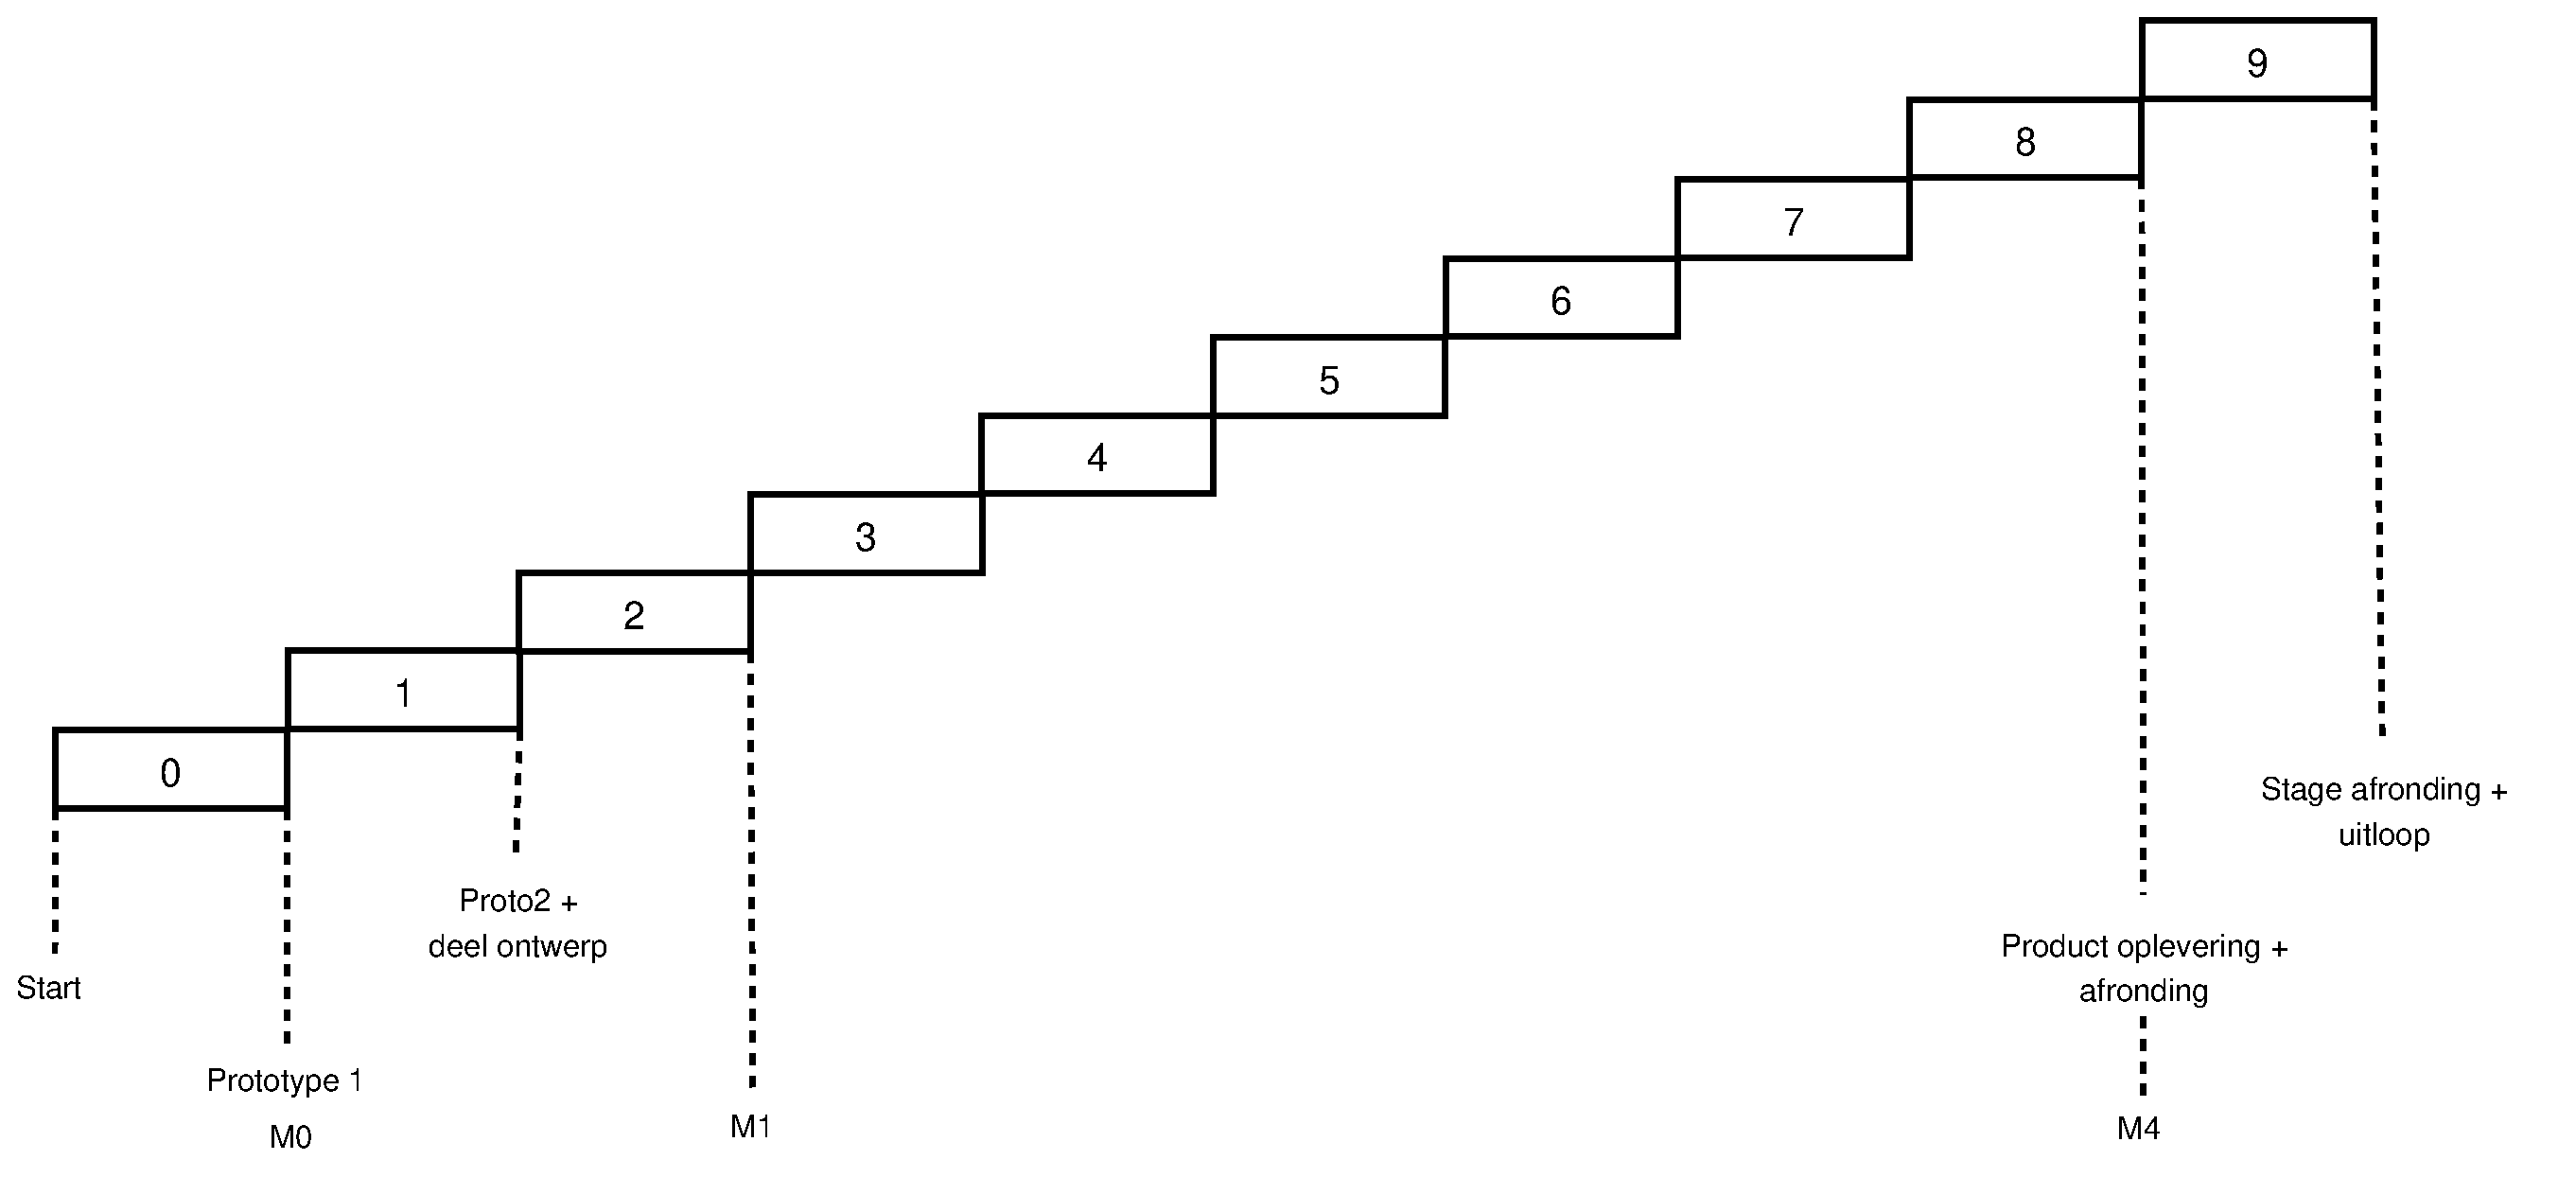
\includegraphics[width=20cm]{planning}
\end{figure}

In dit schema geven de rechthoekige genummerde vakken de increments aan. De gestippelde lijnen geven de gepland afgeronde activiteiten aan en de geplande milestones.

\end{landscape}

\newpage
\subsection{Toelichting}
\index{Planning,toelichting}
\label{planning}

Zoals in de fasering op bladzijde \pageref{fasering} besproken werd, wordt het project ingedeeld in \index{Milestones}milestones. Deze zijn zelf weer opgedeeld in \'e\'en of meerdere \index{Increments}increments.

\begin{tabularx}{\textwidth}{|c|c|X|}
\hline
Increment&Datum&Activiteit\\
\hline
0&2 - 13 Februari&Opstellen en aanpassen Plan van Aanpak, analyses uitvoeren, prototype1\\
\hline
\multicolumn{3}{|l|}{\textbf{Milestone 0: Studie}}\\
\hline
%\hline
%\multicolumn{3}{|l|}{\textbf{Milestone 2: Ontwerp}}\\
%\hline
1&16 - 27 Februari&Prototype2 + deel ontwerp\\
2&1 - 12 Maart&\\
\hline
\multicolumn{3}{|l|}{\textbf{Milestone 1: Voorbereiding}}\\
\hline
3&15 - 26 Maart&\\
%\hline
%\multicolumn{3}{|l|}{\textbf{Milestone 3: Implementatie en testen}}\\
%\hline
4&29 Maart - 9 April&\\
5&12 - 23 April&\\
6&26 April - 7 Mei&\\
7&10 - 21 Mei&\\
8&24 Mei - 4 Juni&Afronden en opleveren product\\
\hline
\multicolumn{3}{|l|}{\textbf{Milestone 4: Product test release}}\\
\hline
9&7 - 18 Juni&Stage afronden, presentatie houden, stageverslag maken\\
\hline
\end{tabularx}

Zoals tijdens de probleemstelling (zie pagina \pageref{probleemstelling}) te zien is, zal al lopende het project extra functionaliteit aangedragen worden. Deze planning zal dan ook aangepast worden.

Het faseringsoverzicht op pagina \pageref{faseringoverzicht} laat zien dat de milestones door elkaar heen lopen. Daarom zijn milestone 2: ontwerp en milestone 3: implementatie en testen niet in deze planning opgenomen.

Tenslotte wil Delem dat ik maximaal \'e\'en dag in de week reserveer voor zaken die niet direct in verband staan met de HSB Bus Analyser, maar waar ik bijvoorbeeld Solutions werk ga doen. Dit omdat er tijdens het werken in een bedrijfssituatie regelmatig iets tussendoor komt wat hogere prioriteit heeft.


% 6. beheersaspecten
\section{Beheersaspecten}

\subsection{Geld}

Delem stelt een maandelijkse stagevergoeding beschikbaar, deze bedraagt \texteuro 406,92 bruto per maand. Verder zal er ook de mogelijkheid om in overleg benodige zaken te kopen.

\subsection{Organisatie}

Zie projectorganisatie op pagina \pageref{organisatie}.

\subsection{Kwaliteit}

In de eerste instantie zal het product zoveel mogelijk door de stagiair zelf getest worden tijdens het ontwikkelen, dit is gebruikelijk binnen Delem. Als de eerste release van het programma vrijgegeven wordt, zullen de gebruikers van het programma hun bevindingen melden, en er indien nodig een PR of CR van maken.

\subsection{Informatie}

Er zal om de week een overleg zijn met de bedrijfsbegeleider, alswel een tweewekelijkse rapportage naar de docentbegeleider.

De software voor het te maken project zal geschreven worden in Microsoft Visual C++ .NET, en moet werken op Windows 2000 en XP machines.

\subsection{Tijd}

De stage duurt tot 18 juni 2004. Op dit tijdstip moet het project afgerond zijn en aan alle formaliteiten voldaan zijn. In geval van ziekte en andere onvoorziene zaken is er eventueel \'e\'en week extra.


% 7. conclusie / aanbevelingen
\chapter{Conclusie}
\index{Conclusie}

Dit verslag bied een overzicht van het verloop van mijn werkzaamheden tijdens mijn $2^e$ stage te Delem BV. Na het gehele verloop van de stage is er een programma gemaakt, waarvan ik hoop dat Delem er veel aan zal hebben. De opzet was het programma zo uitbreidbaar en onderhoudbaar mogelijk te maken, iets wat goed gelukt is.

Tijdens deze stage heb ik, behalve aan de stageopdracht te werken, ook ongeveer \'e\'en dag per week aan andere activiteiten besteed. Een goed voorbeeld hiervan is het testen van een bestaande applicatie VBend\footnote{Virtual Bend, applicatie die een optimale buigvolgorde kan berekenen en simuleren}, waarvan binnenkort een nieuwe versie beschikbaar zou komen. Hierbij ben ik volledig in het projectteam opgenomen en heb ik goed kennis leren maken met de gang van zaken tijdens 'normale' projecten. Ook kwam het gebruik van \index{PR}PR's en \index{CR}CR\footnote{Problem Report/Change Request, zie pagina \pageref{PR} voor meer informatie}'s erg goed naar voren.

Verder heb ik tijdens deze stage heel uitgebreid kennis gemaakt met XML, wat wellicht later nog van pas kan komen. Ook merkte ik dat mijn Windows programmeerkennis niet meer optimaal was (ik gebruik zelf thuis bijna geen Windows), daarin heb ik mezelf ook een stuk meer verdiept.

Ik vind dat ik veel vrijheid heb gehad tijdens het uitoefenen van de stage, ik verwacht dat dit is omdat ik inmiddels al 2 jaar bij de firma Delem werkzaam ben. Hierbij ben ik van mening dat ik nu pas het bedrijf echt goed heb leren kennen, gezien ik eigenlijk pas nu het gevoel heb dat ik weet hoe de projecten daar werken .

Tenslotte denk ik dat dit een geslaagde stage was. Het is goed gedocumenteerd, er is een goed functionerend programma opgeleverd en er zijn al een aantal problemen mee gevonden die wellicht in de toekomst aangepakt zullen worden. Al met al een prima resultaat, wat ook door mijn projectbegeleider bij Delem bevestigd is.



% b. communicatieplan
\chapter{Communicatieplan}

Deze bijlage bevat het communicatieplan, zoals uiteindelijk met de docentbegeleider overeen gekomen. Uiteindelijk bleek het stageverslag eerder af te zijn dan gepland en word daarom ook eerder opgestuurd.

% communicatieplan
\chapter{Communicatieplan}

Deze bijlage bevat het communicatieplan, zoals uiteindelijk met de docentbegeleider overeen gekomen. Uiteindelijk bleek het stageverslag eerder af te zijn dan gepland en word daarom ook eerder opgestuurd.

% communicatieplan
\chapter{Communicatieplan}

Deze bijlage bevat het communicatieplan, zoals uiteindelijk met de docentbegeleider overeen gekomen. Uiteindelijk bleek het stageverslag eerder af te zijn dan gepland en word daarom ook eerder opgestuurd.

% communicatieplan
\input{commplan/commplan.tex}




% c. gebruikte software
\chapter{Gebruikte software}
\index{Gebruikte software}
\label{software}

Hieronder volgt een overzicht van alle gebruikte software, in alfabetische volgorde:

\begin{itemize}
\item ActiveState \index{Perl}Perl (http://www.activestate.com) \\
Perl is een bekende scripttaal. Deze is gebruikt om snel scripts te bouwen om dingen te controleren en zaken om te zetten.
\item \index{dia}dia (http://www.gnome.org/projects/dia/) \\
Dia is een open source diagram editor, die ook onder Win32 werkt. Deze is zeer eenvoudig in het gebruik en kan gewoon als \index{PNG}PNG-files diagrammen exporteren.
\item \index{doxygen}Doxygen (http://doxygen.org) \\
Doxygen is een programma dat aan de hand van commentaar in de sourcecode documentatie van functies en klassen en dergelijke kan genereren. Ik heb het optionele GraphViz (http://www.research.att.com/ sw/tools/graphviz/) programma ook ge\"installeerd, zodat het ook netjes grafische diagrammen genereerde van de klassen.
\item \index{GIMP}GIMP (http:///gimp.org) \\
The GIMP (GNU Image Manipulation Program) is een opensource programma waarmee plaatjes eenvoudig bewerkt kunnen worden. Dit is dan ook gebruikt voor de (zeer minimale) aanpassingen van illustraties in de documentatie.
\item libxml2 (http://xmlsoft.org) \\
Deze open source bibliotheek is oorspronkelijk ontwikkeld voor het Gnome project\footnote{www.gnome.org, een desktop omgeving voor *NIX}. Gelukkig is hij buiten Gnome ook bruikbaar als een stabiele en snelle XML parser. Verder is ook de XSLT processor hiervan, xsltproc.exe, gebruikt om door middel van XSLT de definities om te zetten.
\item \index{MikTeX}MikTeX (http://www.miktex.org) \\
Dit is een Win32 \index{LaTeX}\LaTeX \mbox{ }typesetting programma. Het is gebruikt voor het Plan van Aanpak en dit stageverslag, maar ook de PDF van de gedefinieerde commando's.
\item Microsoft HTML Help Workshop \\
Dit programma is gebruikt om van de HTML uitvoer een CHM helpfile te maken.
\item Microsoft Office 2000 \\
Aangezien niemand bij Delem \LaTeX \mbox{ }gebruikt en het de bedoeling was om de architectuur documenten te kunnen onderhouden, is er voor gekozen dit in standaard Word te doen, dat onderdeel van Microsoft Office is.
\item Microsoft Visual Studio .NET 2003 \\
Deze welbekende C++ omgeving is gebruikt om het programma in te implementeren, met behulp van MFC\footnote{Microsoft Foundation Classes}.
\item Merant Version Manager\footnote{Voorheen bekend onder de naam Primavera Version Manager, deze naam werd nog in het plan van aanpak gebruikt} \\
Dit programma is gebruikt als versie beheer systeem. Alle broncode en documenten staan hierin opgeslagen, evenals oudere versies.
\item Merant Tracker \\
Dit programma is gebruikt om PR-en en CR-en bij te houden.
\item \index{vim}vim (http://www.vim.org) \\
VIM is VI iMproved, een open source editor die erg op vi\footnote{Visual edItor, een zeer standaard UNIX editor} lijkt, maar een hele hoop verbeteringen heeft.
\item \index{Quintessential CD v1.27}Quintessential CD v1.27 (http://www.quinnware.com) \\
Deze Win32 CD speler is erg compact, en vermaakte mij tijdens het uitoefenen van mijn stageactiviteiten.
\item \index{zsh}zsh (http://www.zsh.org) \\
De Z Shell is een open source shell, die werkt op *NIX en Win32 machines. Deze is veel krachtiger dan de standaard Microsoft shell en werd daarom gebruikt in plaats van de laatste.
\end{itemize}


% index
\backmatter
\printindex

\end{document}
